\documentclass[portrait,a1paper,fontscale=0.46]{baposter}

\usepackage{calc}
\usepackage{graphicx}
\usepackage{amsmath}
\usepackage{amssymb}
\usepackage{relsize}
\usepackage{multicol}
\usepackage{multirow}
\usepackage{rotating}
\usepackage{bm}
\usepackage{url}
\usepackage{color}

\usepackage{graphicx}
\usepackage{multicol}
\usepackage[font=scriptsize,labelfont=bf]{caption}

\begin{document}

\begin{poster}{
  grid=false,
  columns=4,
  colspacing=1em,
  bgColorOne=white,
  bgColorTwo=white,
  borderColor=blue,
  headerColorOne=black,
  headerColorTwo=blue,
  headerFontColor=white,
  boxColorOne=white,
  boxColorTwo=blue,
  textborder=roundedleft,
  eyecatcher=true,
  headerborder=closed,
  headerheight=0.1\textheight,
  headershape=roundedright,
  headershade=shadelr,
  headerfont=\Large\bf\textsc,
  textfont={\setlength{\parindent}{1.5em}},
  boxshade=plain,
  background=plain,
  linewidth=2pt
  }
  {
\includegraphics[width=18em]{Poster-images/7971.jpg}}
  % Title
  {\bf\textsc{Analysis of the BioModels Database}\vspace{0.5em}}
  % Authors
  {\textsc{\{ James Hollins * \& Colin Gillespie \}}}
  
 \headerbox{Biomodels Database}{name=biomodelsdatabase,column=0,row=0}{
 \begin{multicols}{2}{
 Biomodels Database is an online resource for storing and serving quantative models of biomedical  interest. 
  
 {\flushleft{
\includegraphics[scale=0.7]{Poster-images/Biomodels_logo.png}}}
 }
 The database was created in 2005.
 \end{multicols}
 \vspace{-0.5em}
 The focus of the project is the curated branch of the database. Following the release on 11th August, there are 424 models in this branch, which have all been described in peer reviewed scientific literature.
 }
  
  \headerbox{R}{name=r, column=1,row=0}{
  \begin{multicols}{2}{
  R is a language and environment for statistical computing and graphics, providing a wide variety of statistical 

  {\flushleft{
\includegraphics[trim= 0.9mm 0mm 0.9mm 1.7mm, clip,scale=0.1326]{Poster-images/Rlogo.pdf}}}
  }
  and graphical techniques.
  
  \end{multicols}
  \vspace{-0.5em}
  R is extensible by installing packages. An example is the package rsbml used to parse and extract information from SBML files. However, only 357 of the 424 curated models could be parsed in R using this package.
  
  }
  
  \headerbox{Models and Species over Time}{name=modelsnspecs,column=2,span=2}{
 \begin{multicols}{2}
 {\flushleft{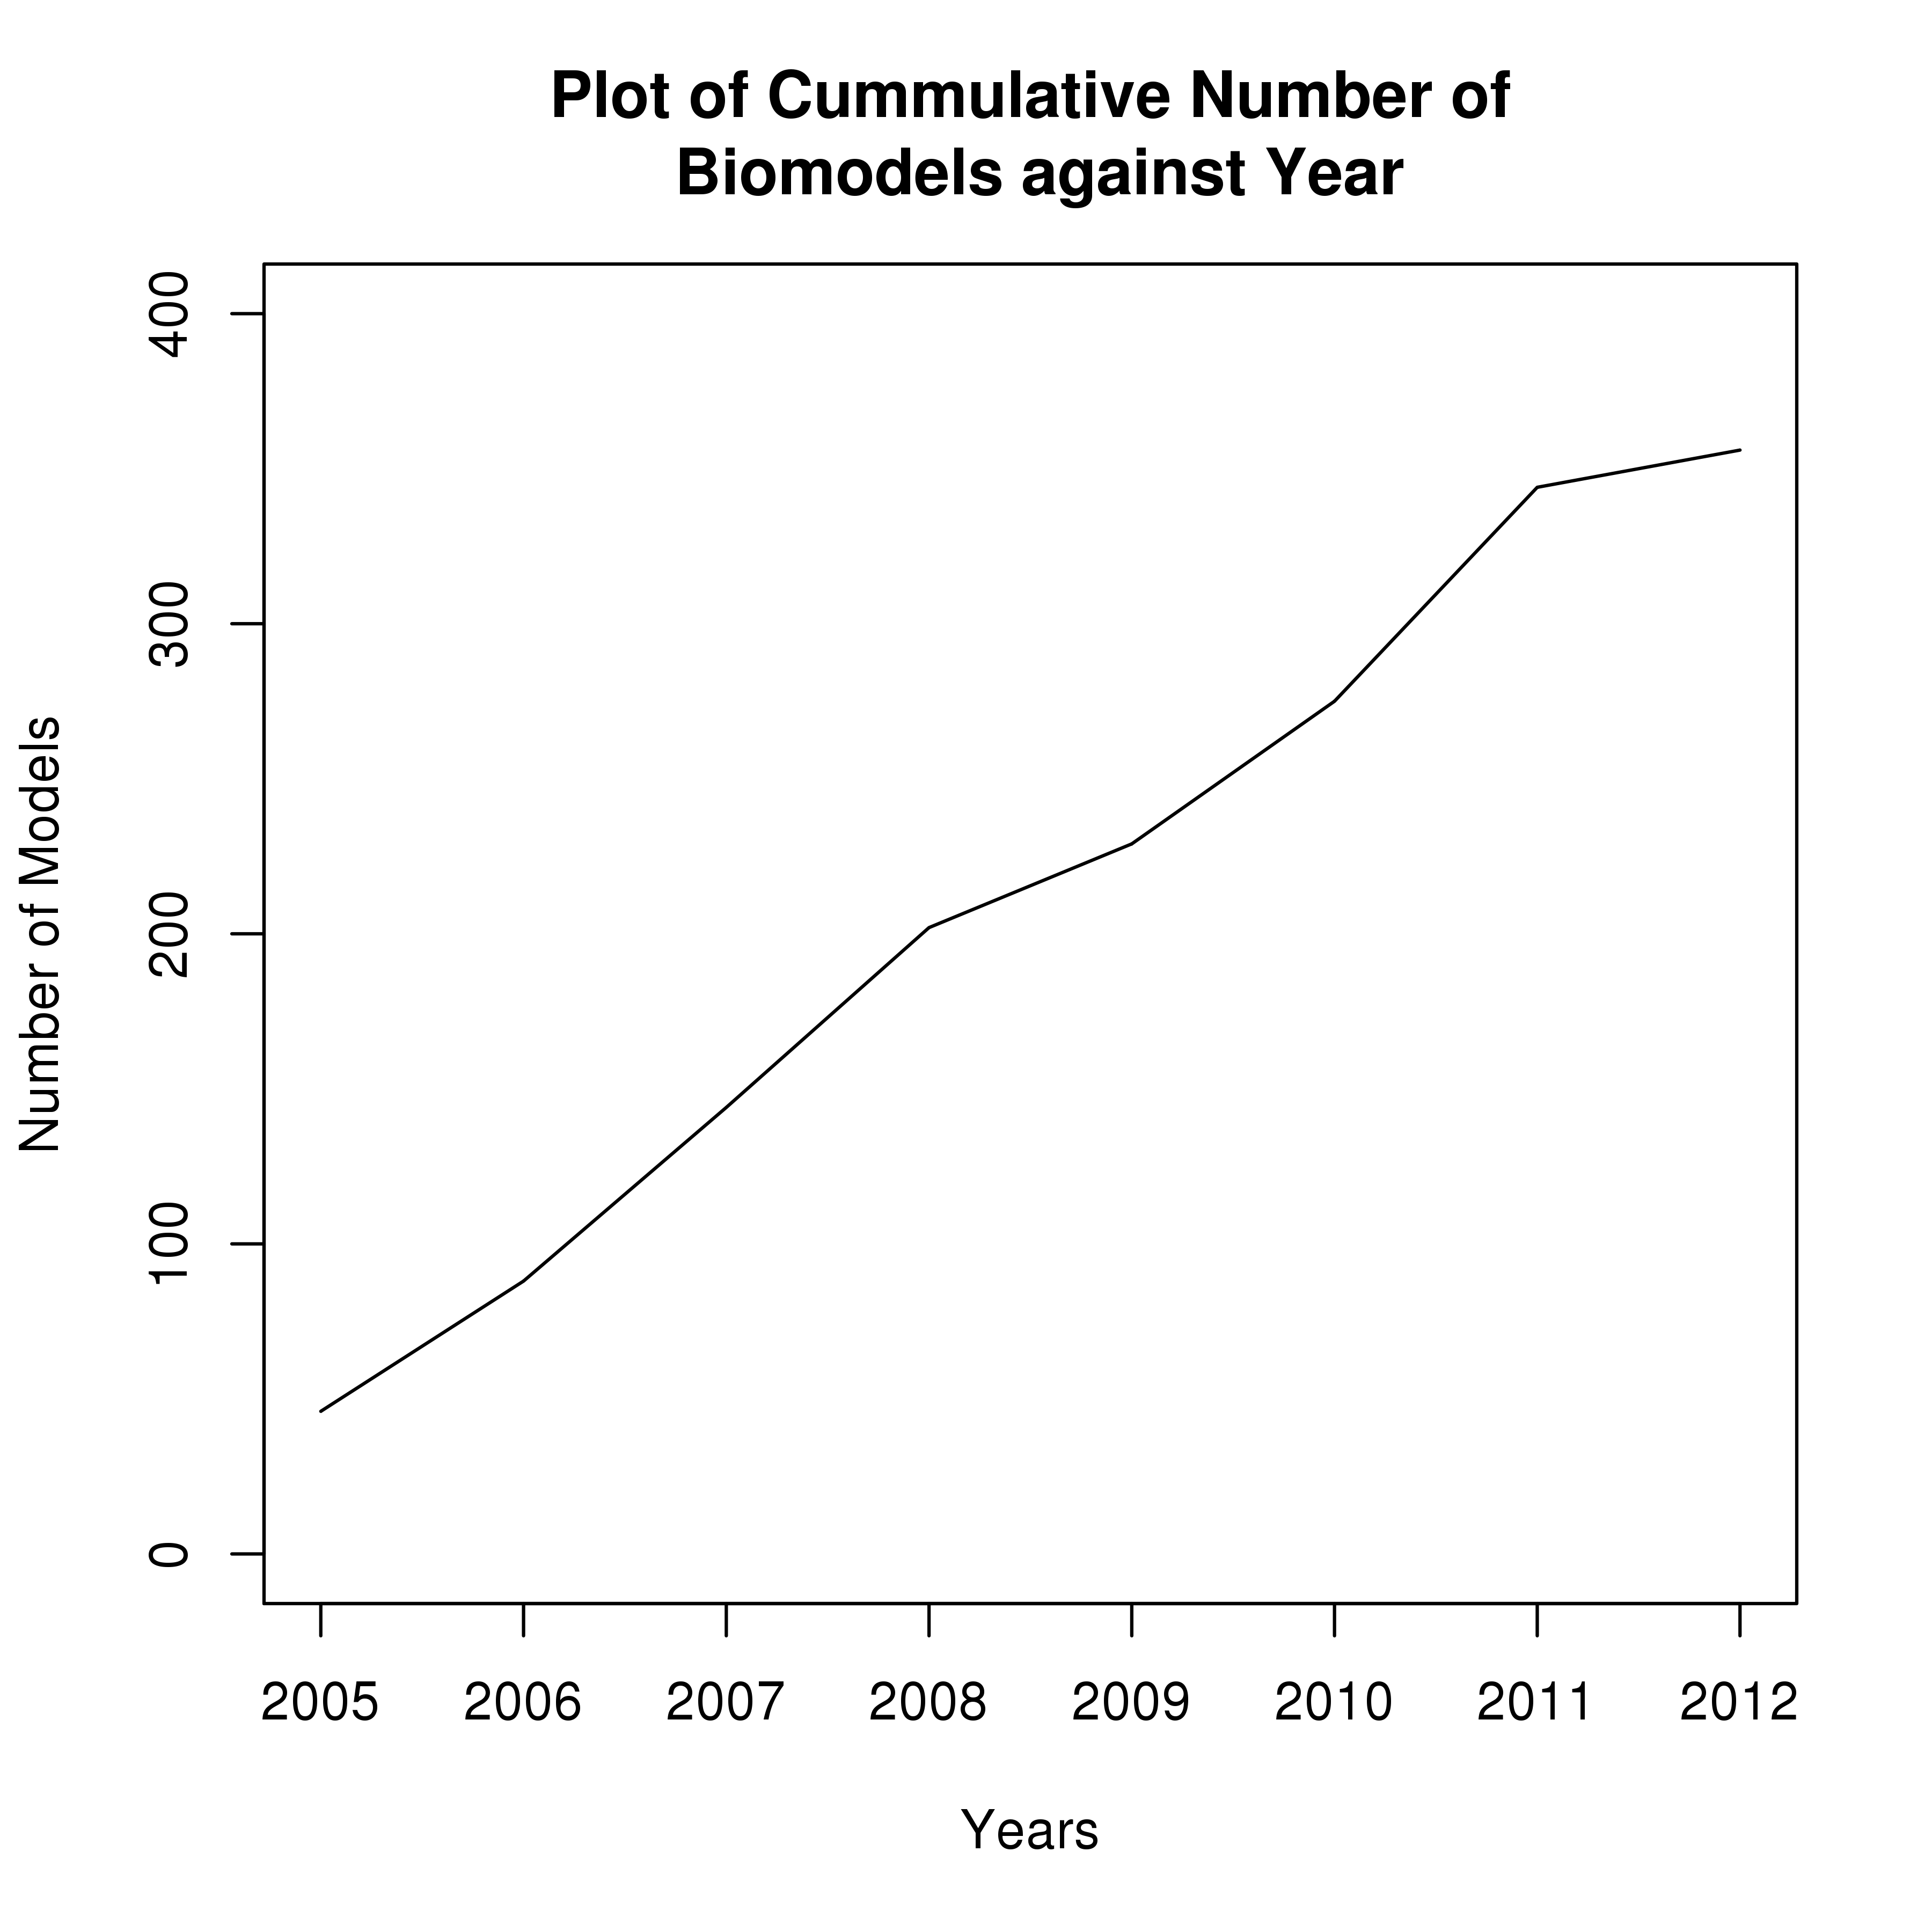
\includegraphics[trim= 1.5mm 5mm 5mm 4.5mm, clip, scale=0.42]{Poster-images/CummulativeModelsPlot.png}}}
 
 The increase in the number of curated models appears to be almost linear, suggesting that models are being added at a reasonably constant rate.
 
 {\flushleft{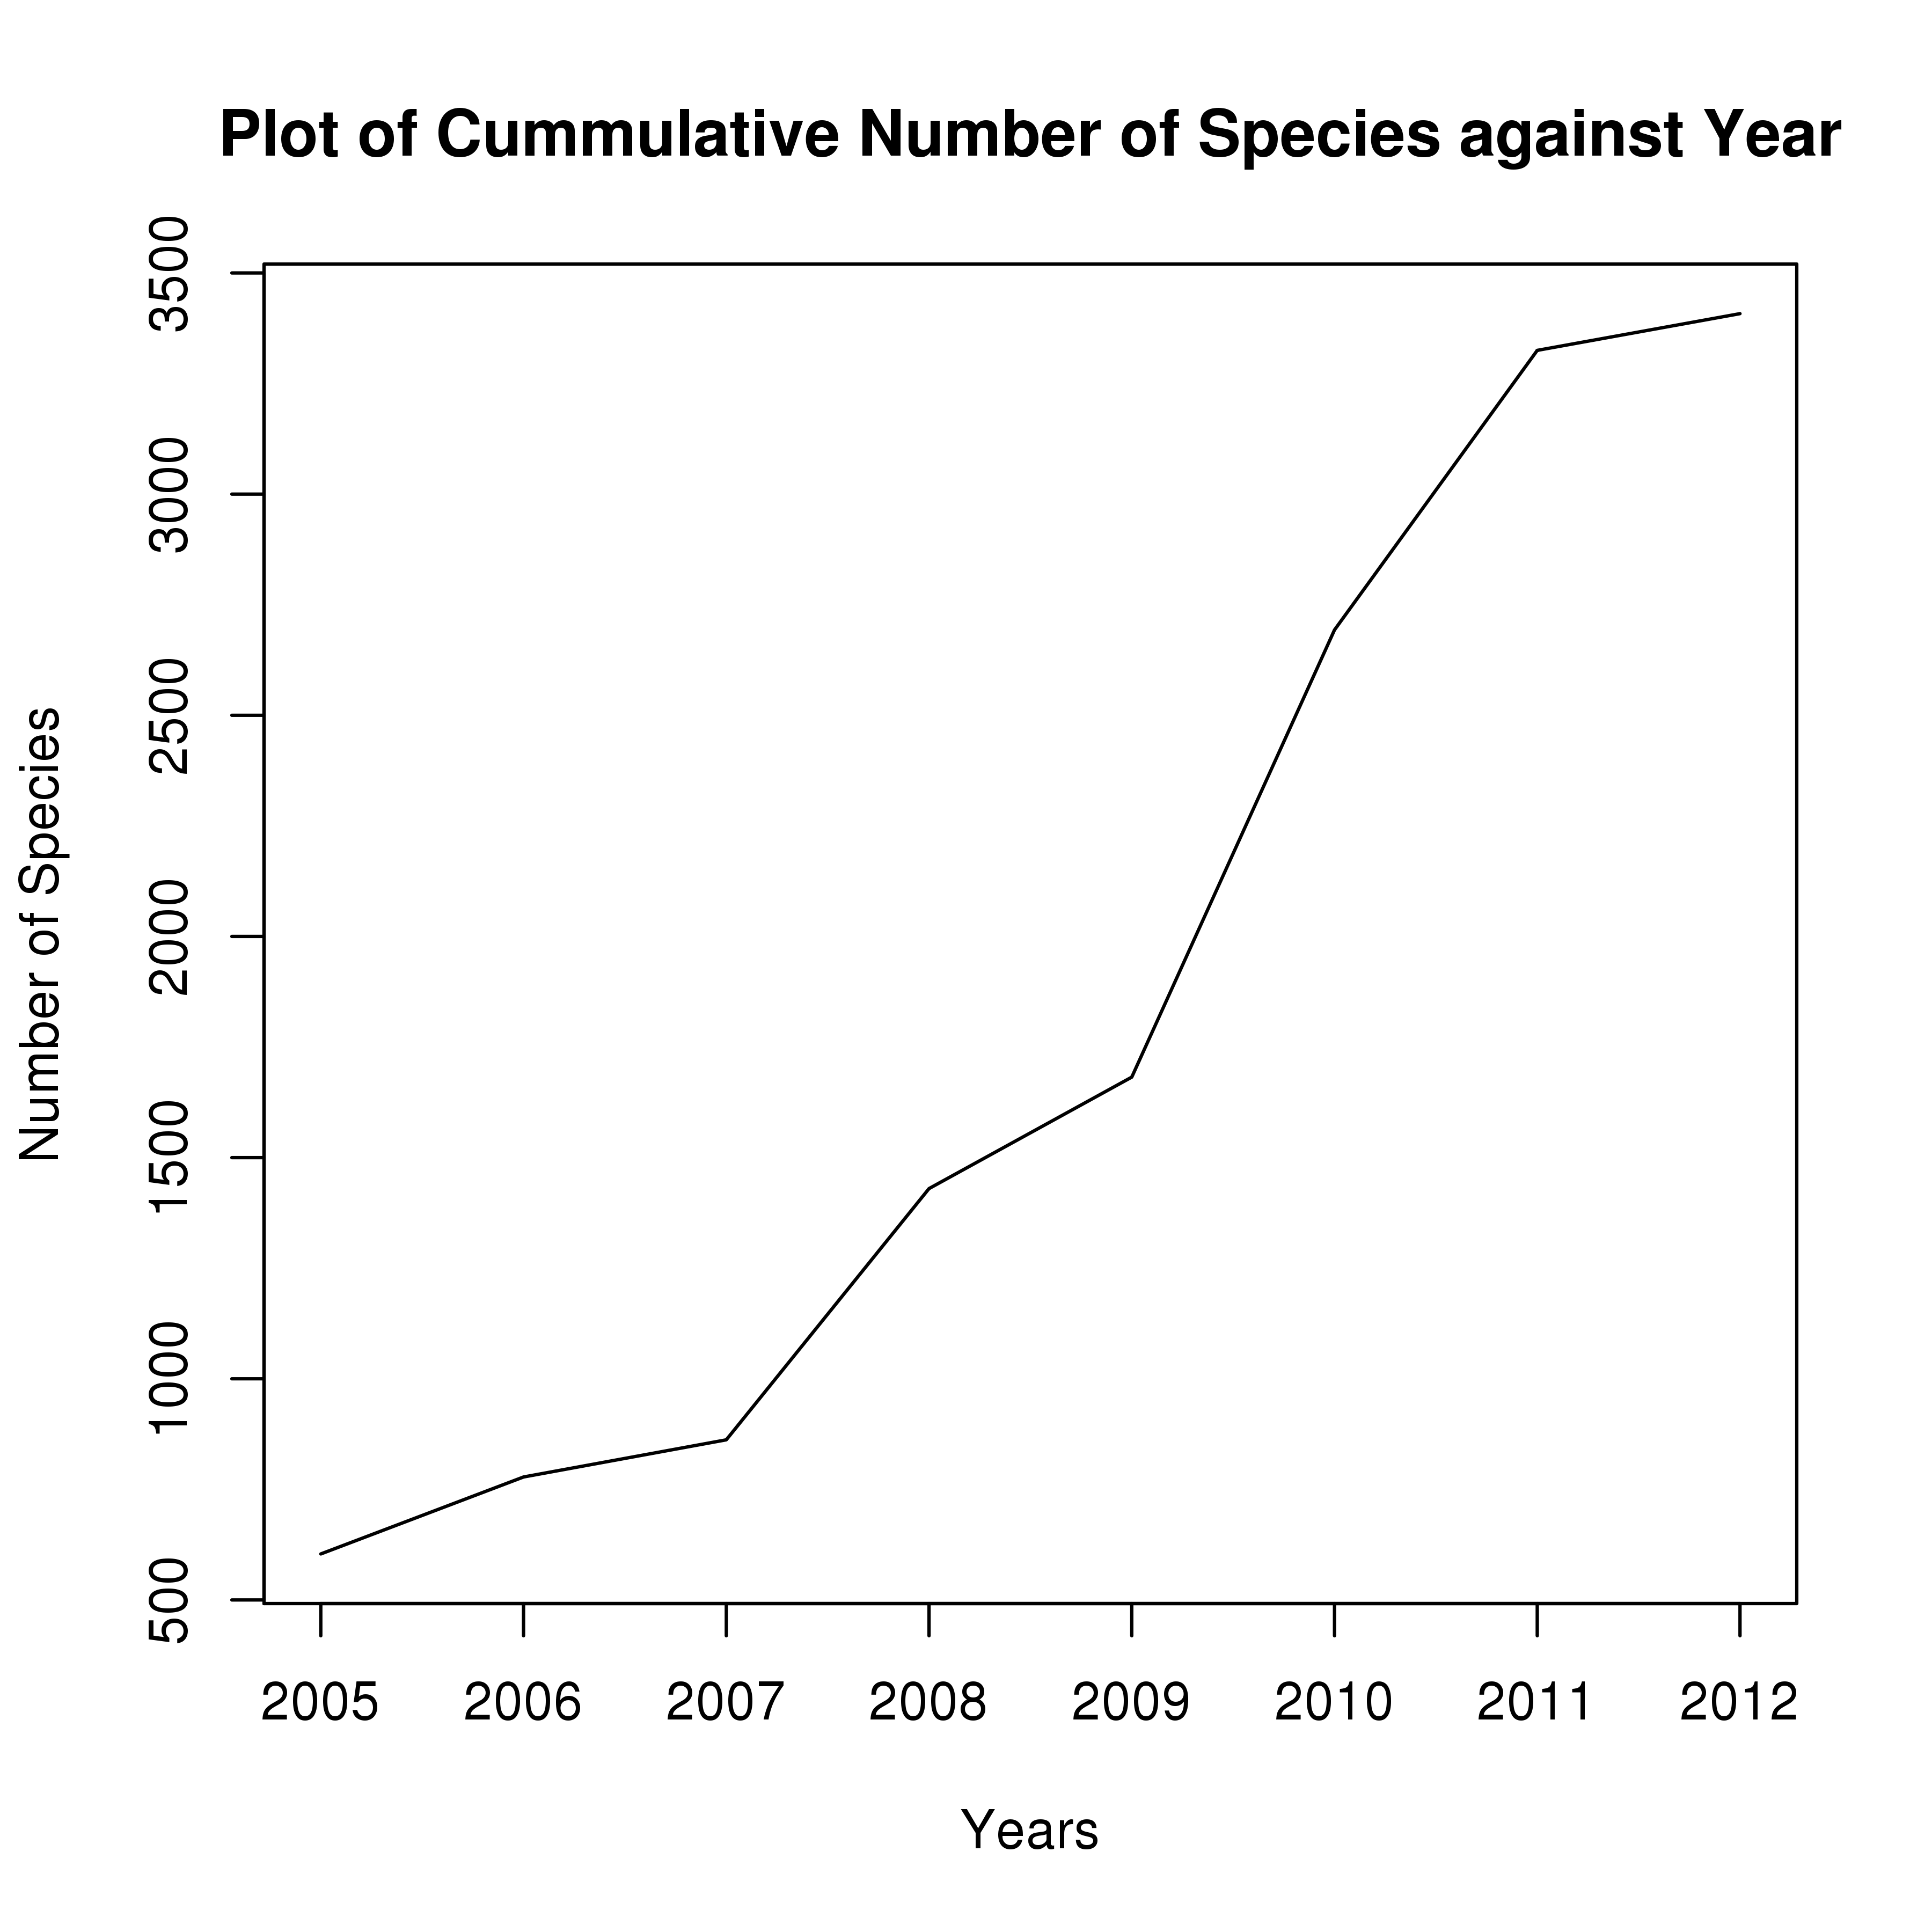
\includegraphics[trim= 1.5mm 5mm 5mm 4.5mm, clip, scale=0.42]{Poster-images/CummulativeSpeciesPlot.png}}}
 
 As shown above, there appears to be a pattern that a large increase in the number of species in one year precedes a smaller increase in the next year.

 \end{multicols}
 }

 \headerbox{References}{name=sboterms,column=0, span=2,above=bottom}{  
  \smaller
  \vspace{-0.4em}
  \bibliographystyle{ieee}
  \renewcommand{\section}[2]{\vskip 0.05em}
  \begin{thebibliography}{1}\itemsep=-0.01em
    \setlength{\baselineskip}{0.4em}
    \bibitem{biochem}
      Wolkenhauer,~O., Wellstead,~P., Cho,~K.H.
      \newblock Essays in Biochemistry volume 45 Systems Biology
    \bibitem{systemsbiology}
      Wilkinson,~D.
      \newblock Stochastic Modelling for Systems Biology
    \bibitem{biomodels}
      BioModels Database
      \newblock $~~$ ({\em http:$//$www.ebi.ac.uk$/$biomodels$-$main$/$})
    \bibitem{rproject}
      R Project
      \newblock $~~$ ({\em http:$//$www.r$-$project.org$/$}) 
    \end{thebibliography}
  }
  
  \headerbox{Parameters}{name=paras,column=2,span=2,above=bottom}{
 \begin{multicols}{2}
 {\flushleft{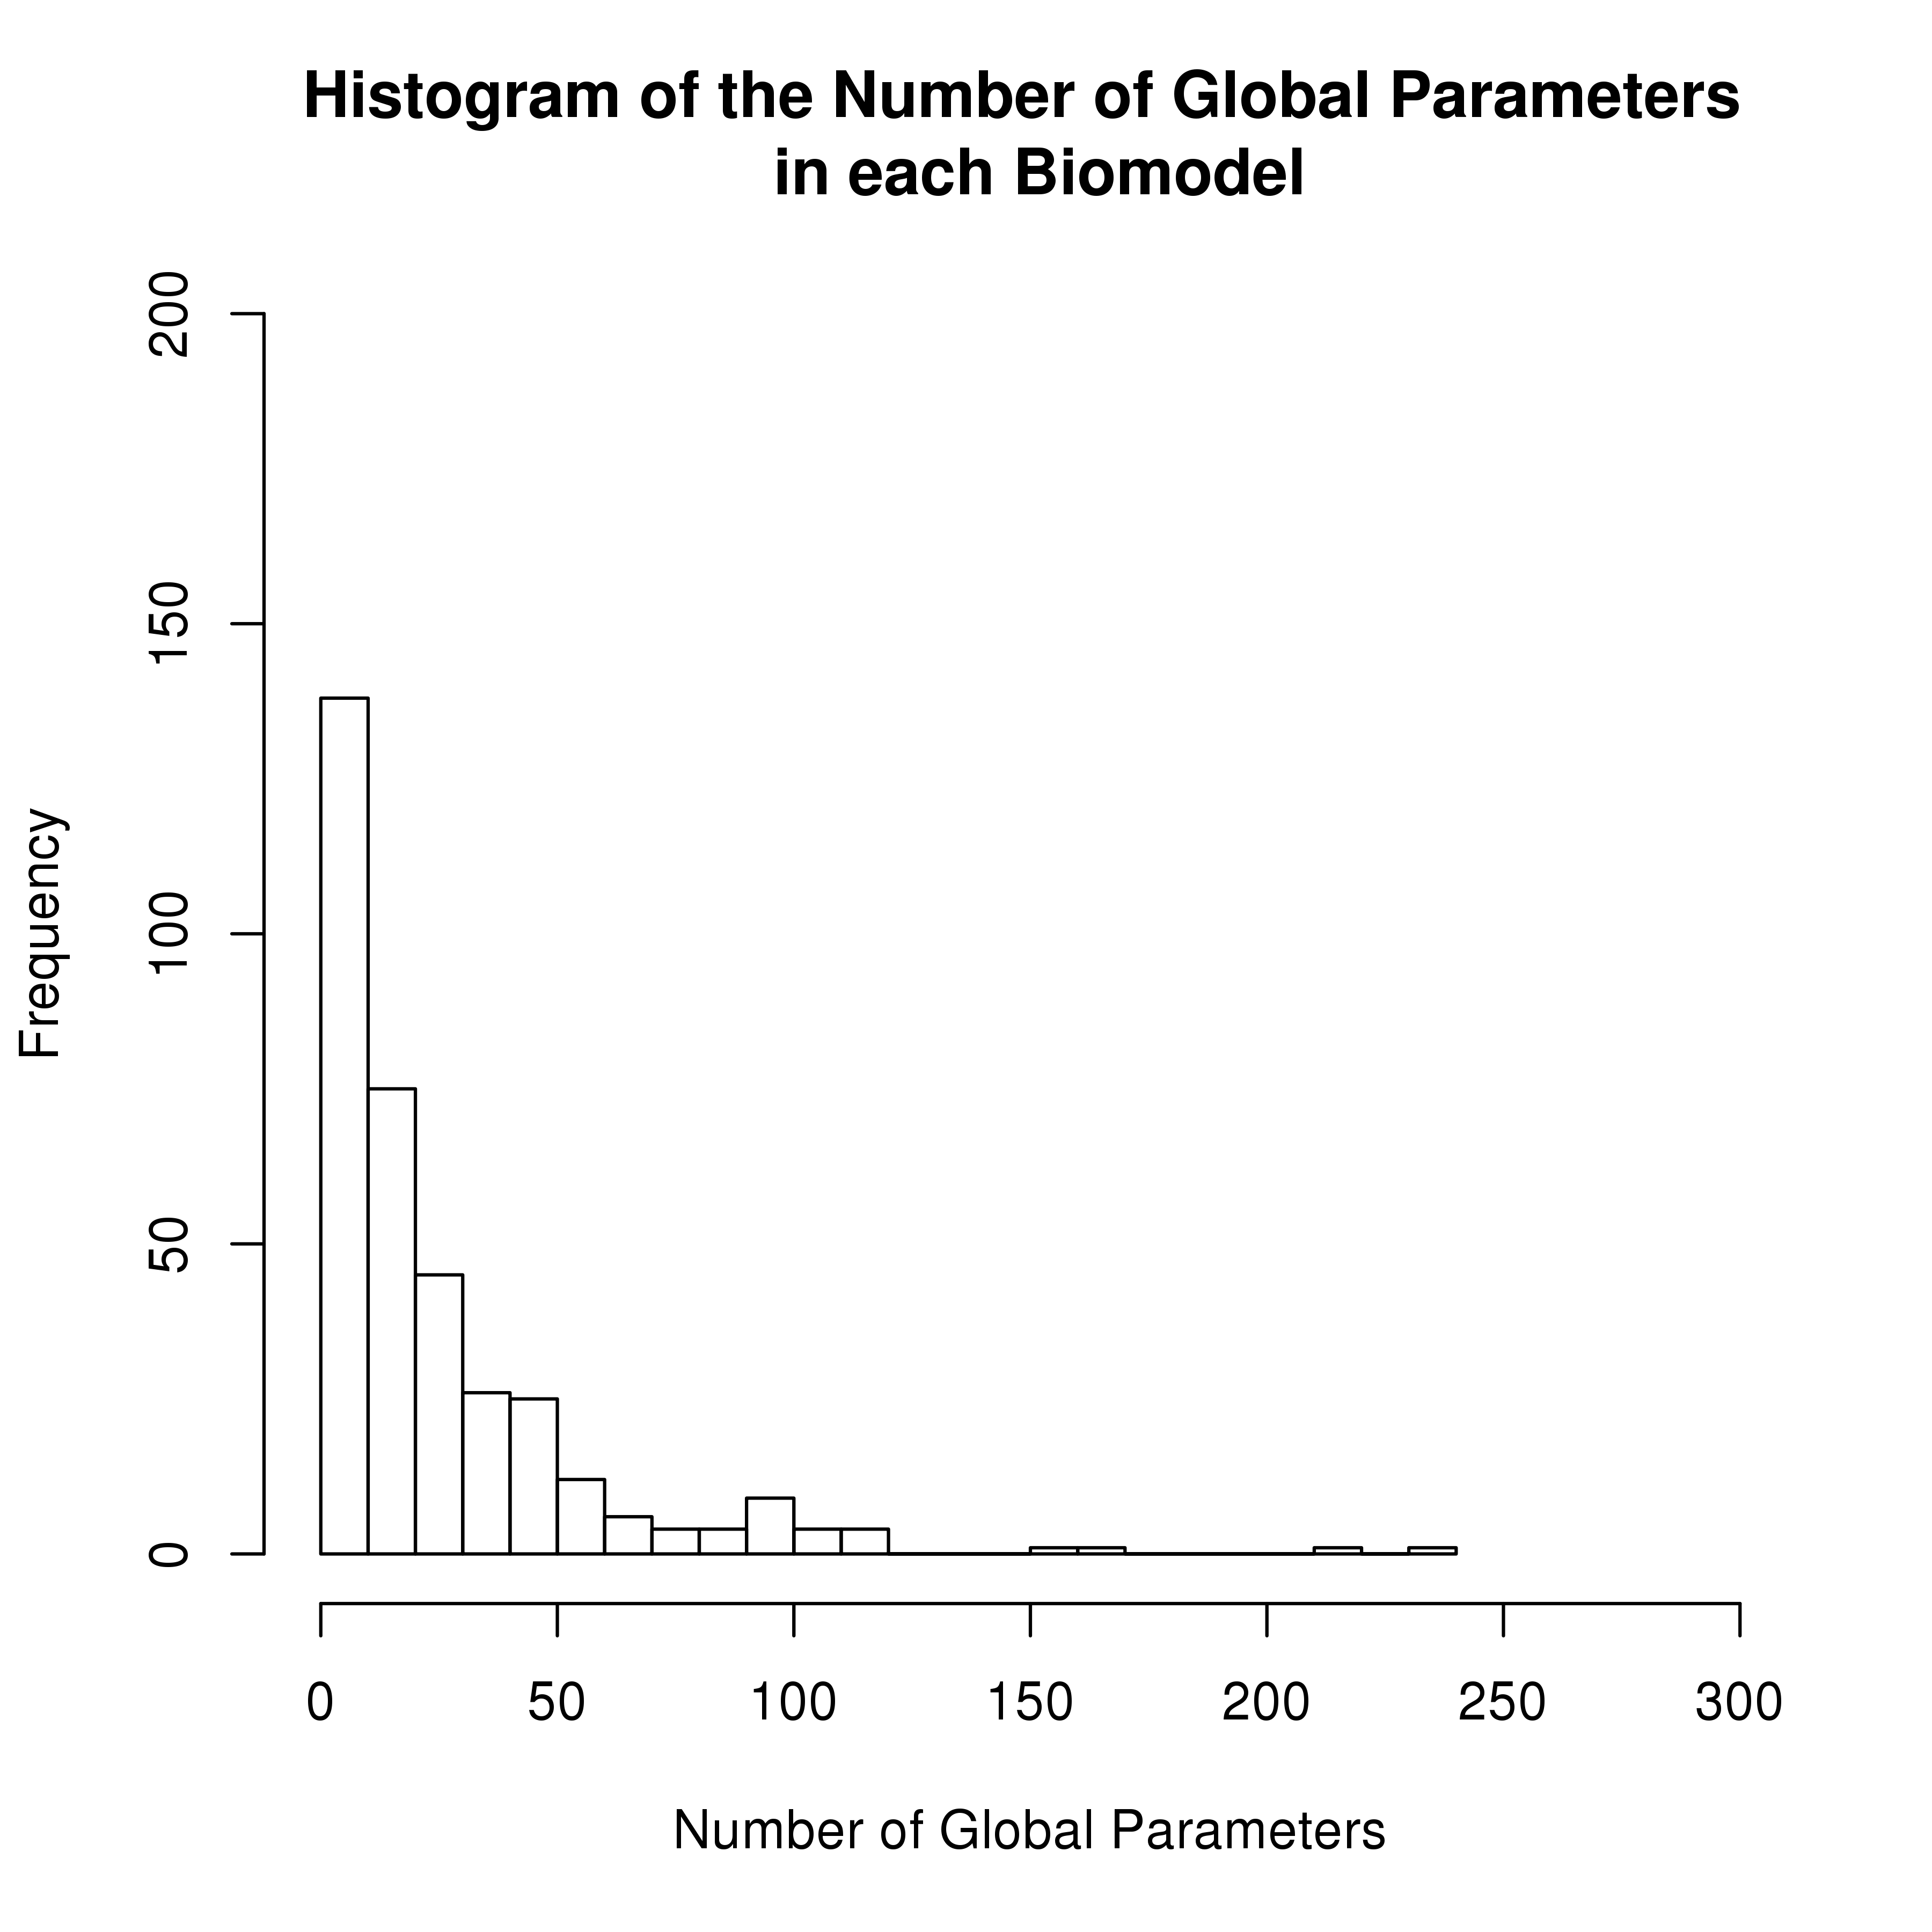
\includegraphics[trim= 1.5mm 5mm 5mm 5mm, clip, scale=0.42]{Poster-images/GlobalParametersHistogram.png}}}
  
  The majority of models have 20 or less global parameters. This suggests that the models tend to have a low number of global parameters.

 
 {\flushleft{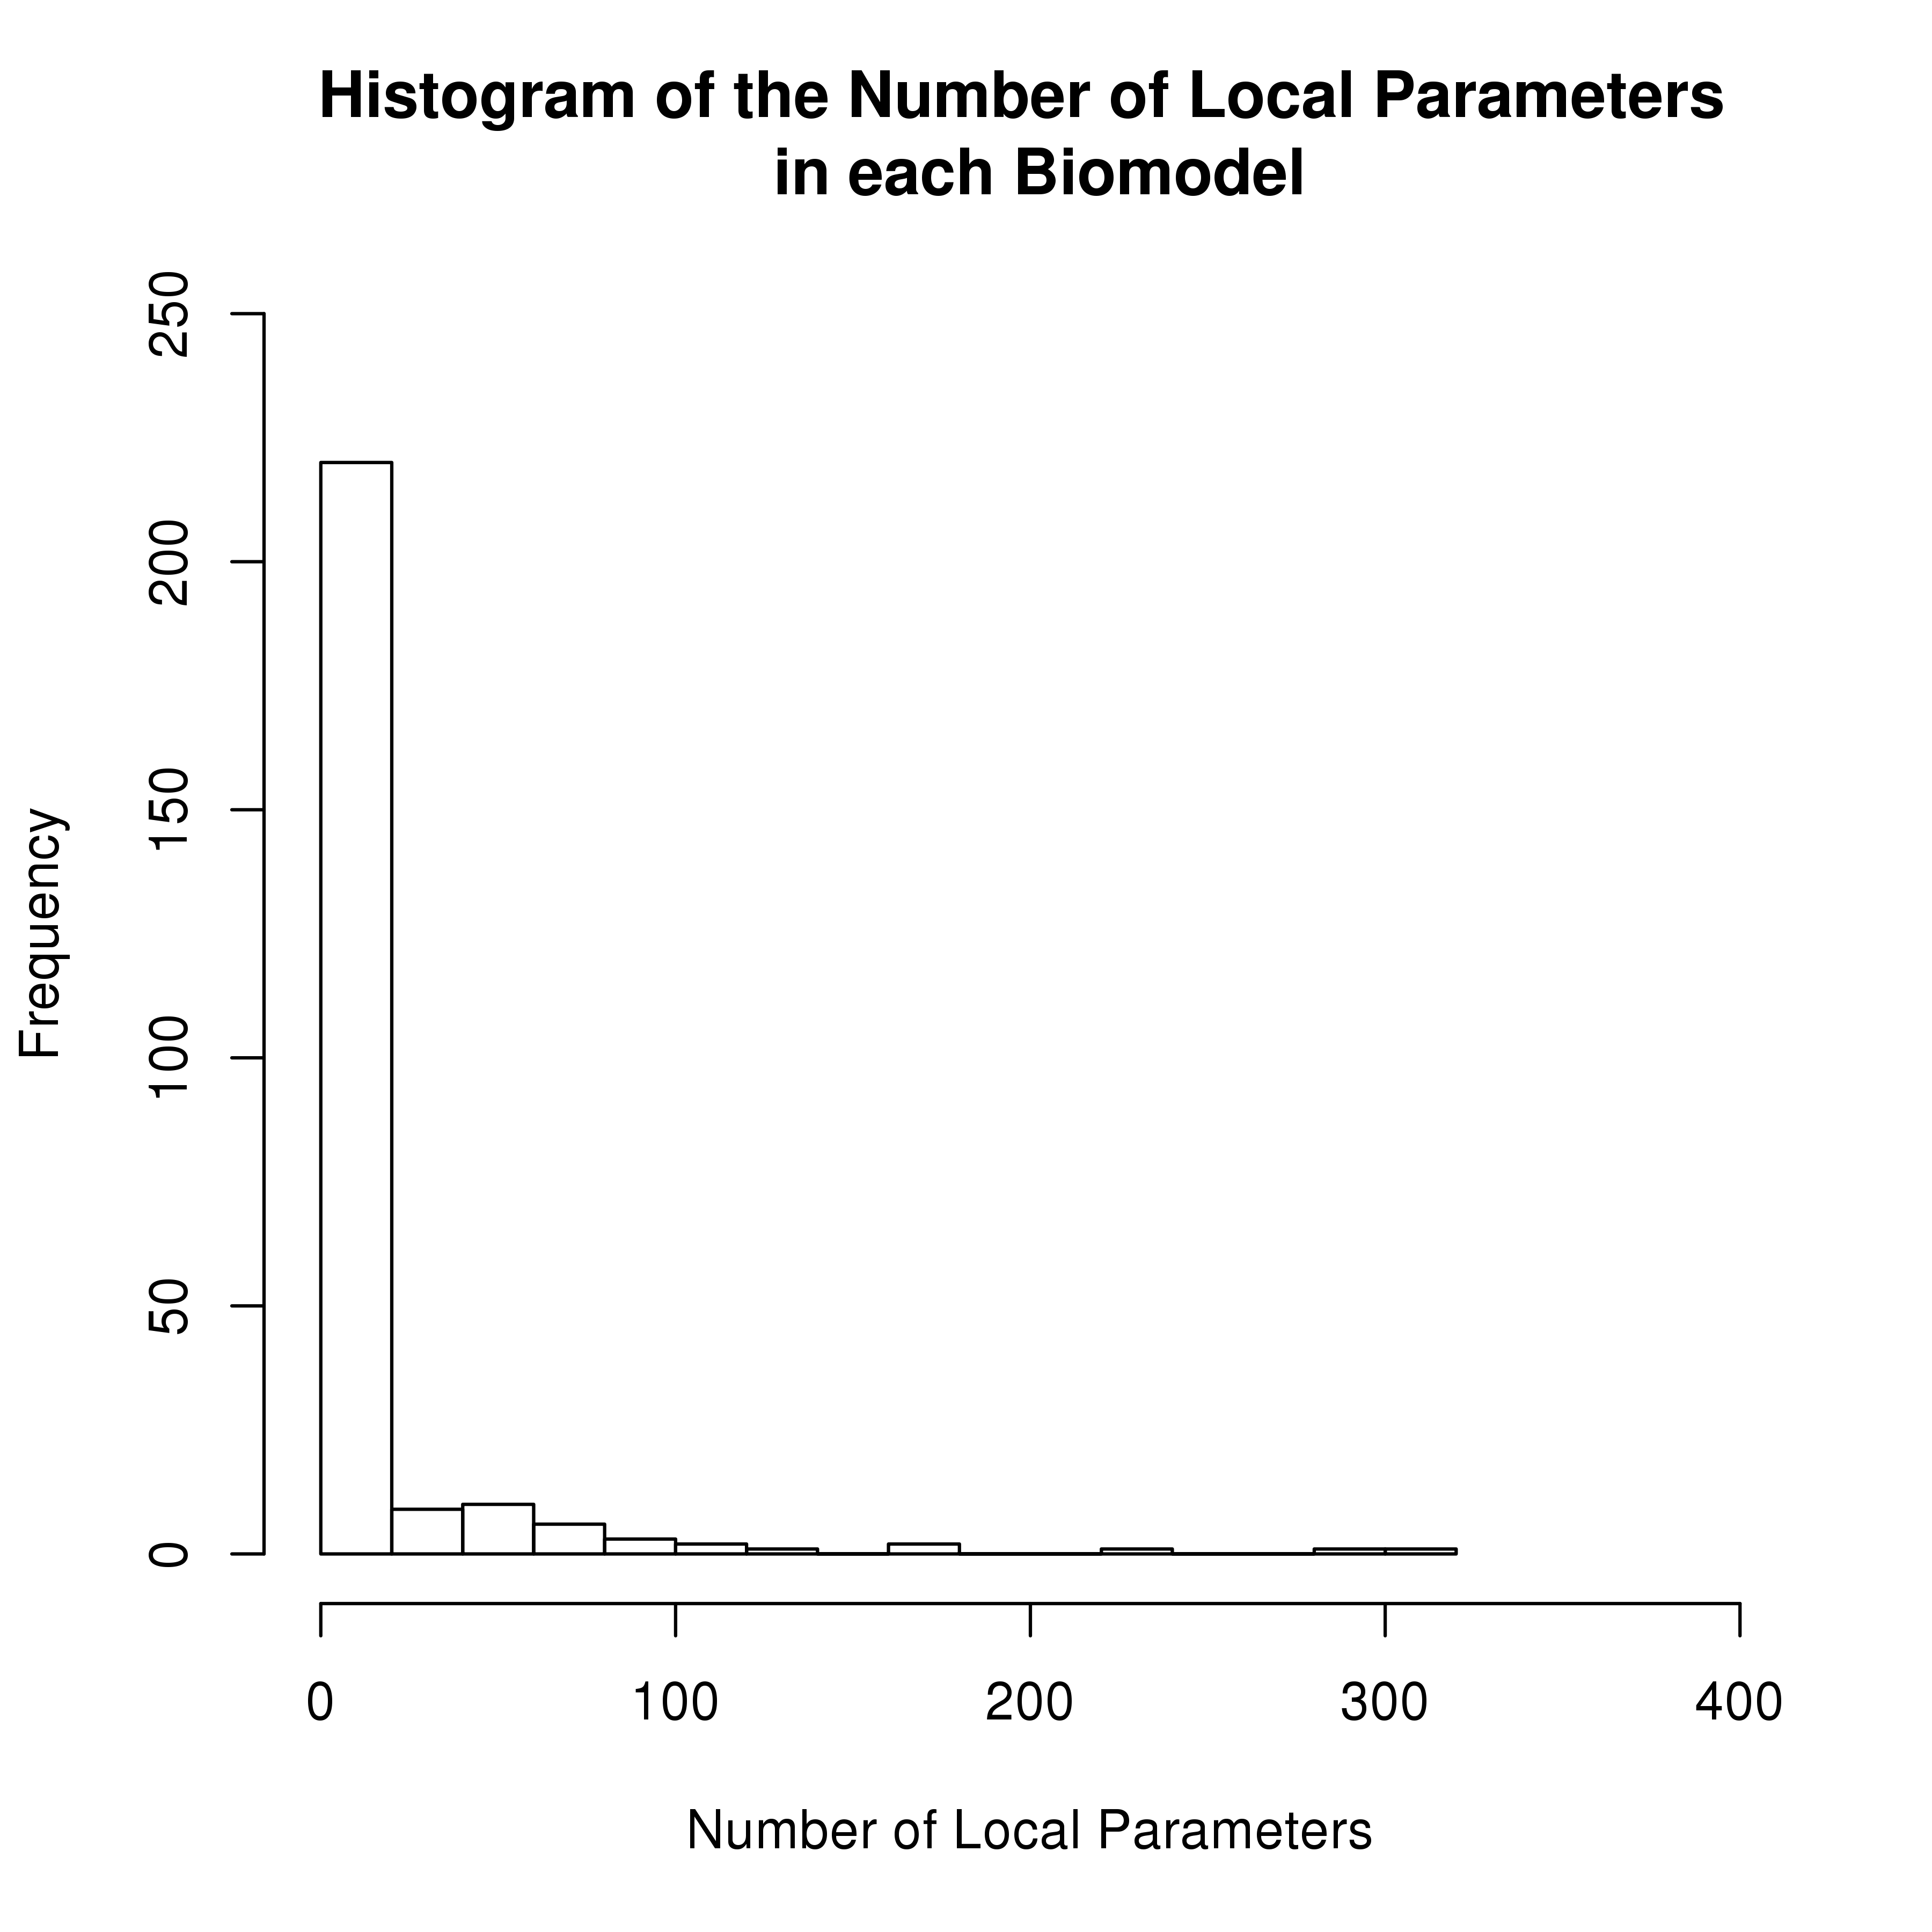
\includegraphics[trim= 1.5mm 5mm 5mm 5mm, clip, scale=0.42]{Poster-images/LocalParametersHistogram.png}}}
 
 The majority of models have 10 or less local parameters. This suggests that the models tend to have a low number of local parameters.
 \end{multicols}
 }
 
 \headerbox{SBML}{name=sbml,column=0,span=2,below=r}{
 \begin{multicols}{2}
 SBML is a modelling standard used for exchanging models between different software tools. An example of SBML code is shown below:
 
 
\includegraphics[scale=0.6]{Poster-images/sbml.png}
 \end{multicols}
 
 \vspace{-2.0em}
 \begin{flushleft}
 {\scriptsize{
  \color{blue}
 <\color{red}listOfSpecies\color{blue}>
 
 <\color{red}species metaid$\color{blue}=$\color{blue}"$\color{black}\_230475$\color{blue}" \color{red} id$\color{blue}=$\color{blue}"\color{black}C\color{blue}" \color{red} name$\color{blue}=$\color{blue}"\color{black}Cyclin\color{blue}" \color{red} compartment$\color{blue}=$\color{blue}"\color{black}cell\color{blue}" \color{red} initialConcentration$\color{blue}=$\color{blue}"$\color{black}0.01$\color{blue}" \color{red} substanceUnits$\color{blue}=$\color{blue}"\color{black}substance\color{blue}" \color{red} sboTerm$\color{blue}=$\color{blue}"\color{black}SBO:$0000252$\color{blue}"/>
 
 <\color{red}species metaid$\color{blue}=$\color{blue}"$\color{black}\_230495$\color{blue}" \color{red} id$\color{blue}=$\color{blue}"\color{black}M\color{blue}" \color{red} name$\color{blue}=$\color{blue}"\color{black}CDC-2 Kinase\color{blue}" \color{red} compartment$\color{blue}=$\color{blue}"\color{black}cell\color{blue}" \color{red} initialConcentration$\color{blue}=$\color{blue}"$\color{black}0.01$\color{blue}" \color{red} substanceUnits$\color{blue}=$\color{blue}"\color{black}substance\color{blue}" \color{red} sboTerm$\color{blue}=$\color{blue}"\color{black}SBO:$0000252$\color{blue}"/>
 
 <\color{red}species metaid$\color{blue}=$\color{blue}"$\color{black}\_230515$\color{blue}" \color{red} id$\color{blue}=$\color{blue}"\color{black}X\color{blue}" \color{red} name$ \color{blue}=$ \color{blue} "\color{black}Cyclin Protease\color{blue}" \color{red} compartment$\color{blue}=$\color{blue}"\color{black}cell\color{blue}" \color{red} initialConcentration$\color{blue}=$\color{blue}"$\color{black} 0.01$\color{blue}" \color{red} substanceUnits$\color{blue}=$\color{blue}"\color{black}substance \color{blue}" \color{red} sboTerm$\color{blue}=$\color{blue}"\color{black}SBO:$0000297$\color{blue}"/>
 
 \vspace{-0.5em}
 <\color{red}/listOfSpecies\color{blue}>}}
 \end{flushleft}
 
 SBML represents the models as a list of chemical transformations, since every biological process in a cell can be described as a series of reactions
 
 SBML is easy for computers to generate and parse but difficult for humans to read and write. Hence, R was used since R is easier to work with than SBML. 
 }
 
 \headerbox{Terms}{name=terms,column=0,span=2,below=sbml}{
 \begin{multicols}{2}
 Consider we have a chemical called X. Let there be a model describing the rate of change of X by the following equation:\\
 
 $\frac{dX(t)}{dt} = -k_1 X(t) + k_2$\\
 
 Where the amount of X is altered by the following processes:\\
 
 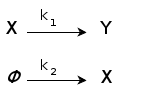
\includegraphics[scale=0.5]{Poster-images/TermDiagram.png}
 
 \begin{itemize}
 \item The entities X and Y are species. Species range from chemicals such as ions or molecules to biological entities such as protein binding sites.
  
 \item The process altering the amount of X are reactions. Reactions are any processes by which the amounts of the species in a model change.
 
 \item $k_1$ and $k_2$ are parameters. Parameters are the numbers used in the desrciption of the rate laws of reactions.
 
 \end{itemize}
 \end{multicols}
 }
 
  \headerbox{Connections}{name=connections,column=0,below=terms}{
 In the project, a species has a 'connection' for each reaction in which the species is present.
 
 Consider the following set of reactions:
 
 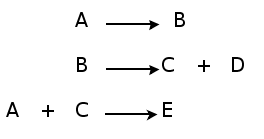
\includegraphics[scale=0.4]{Poster-images/connectiondrawing.png}
 
 Since A, B and C each appear in 2 reactions, they each have 2 connections. D and E each appear in just 1 reaction and so have just 1 connection.
 
 The average number of connections per species in the database is 5.7226 (to 4 decimal places). 
 }
 
 \headerbox{SBO Terms}{name=sboterms,column=1,below=terms}{
 Systems Biology Ontology (SBO) terms are used to provide additional information about model constituents.

 The possibility of using SBO terms to track which models certain species apperared in was explored. However, it was found that species do not necessarily have unique SBO terms 

  \vspace{-1.0em}
  {\flushleft{
  \footnotesize{
    \captionof{table}{Species SBO terms from one model}
      \label{tab:name}
      \begin{tabular}{ | p{1.5cm} | p{2.0cm} | p{1.05cm} | }
    \hline
    sboTerm & Model ID & Frequency \\ \hline
    SBO:0000297 & $\text{\textnormal{EPSP\_Edelstein}}$ & 8 \\ \hline
    SBO:0000420 & $\text{\textnormal{EPSP\_Edelstein}}$ & 4 \\
    \hline
    \end{tabular}}}}
  
  \vspace{1.0em}
  Similar problems were found in each model. Therefore, it is not possible to use SBO terms to track where species appear.
}
 
 \headerbox{Species and Reactions}{name=specsnreacts,column=2,row=0,span=2,below=modelsnspecs}{
 \begin{multicols}{2}
 {\flushleft{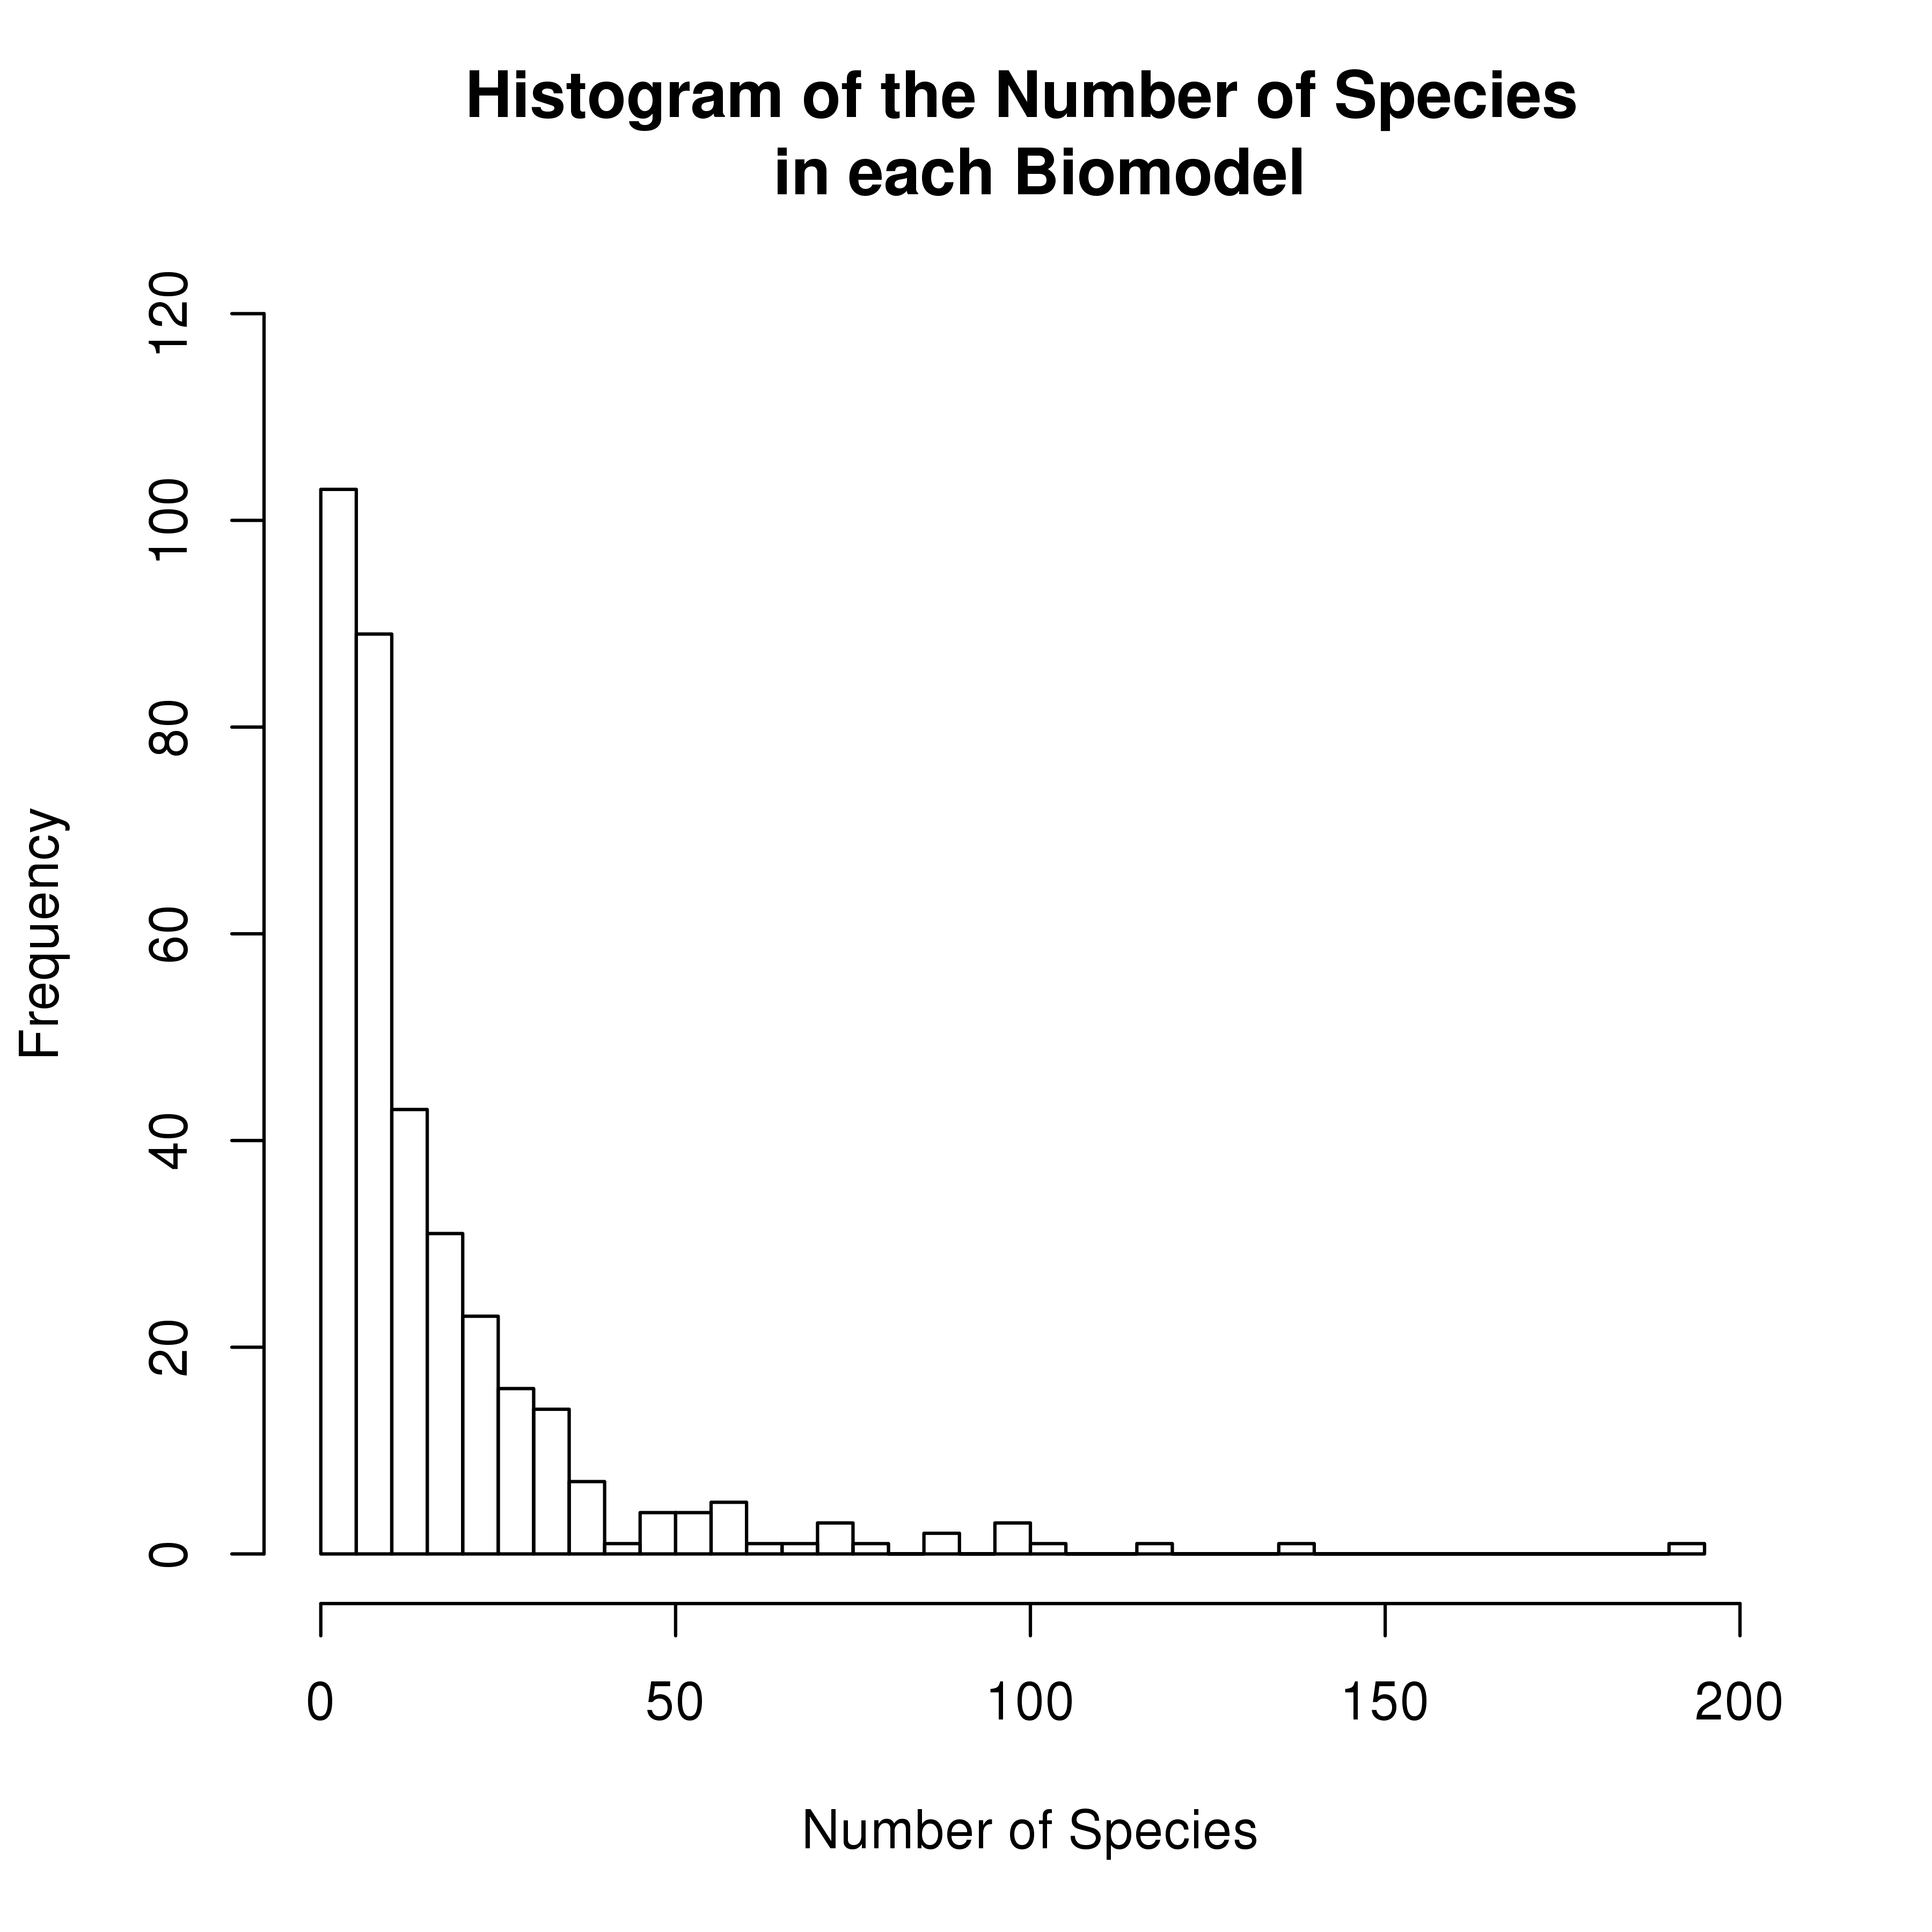
\includegraphics[trim= 1.5mm 5mm 5mm 5mm, clip, scale=0.42]{Poster-images/SpeciesHistogram.png}}}
 
 As shown in the graph above, the majority of models have 10 or less species, suggesting that the models tend to have small numbers of species. \\
 
 {\flushleft{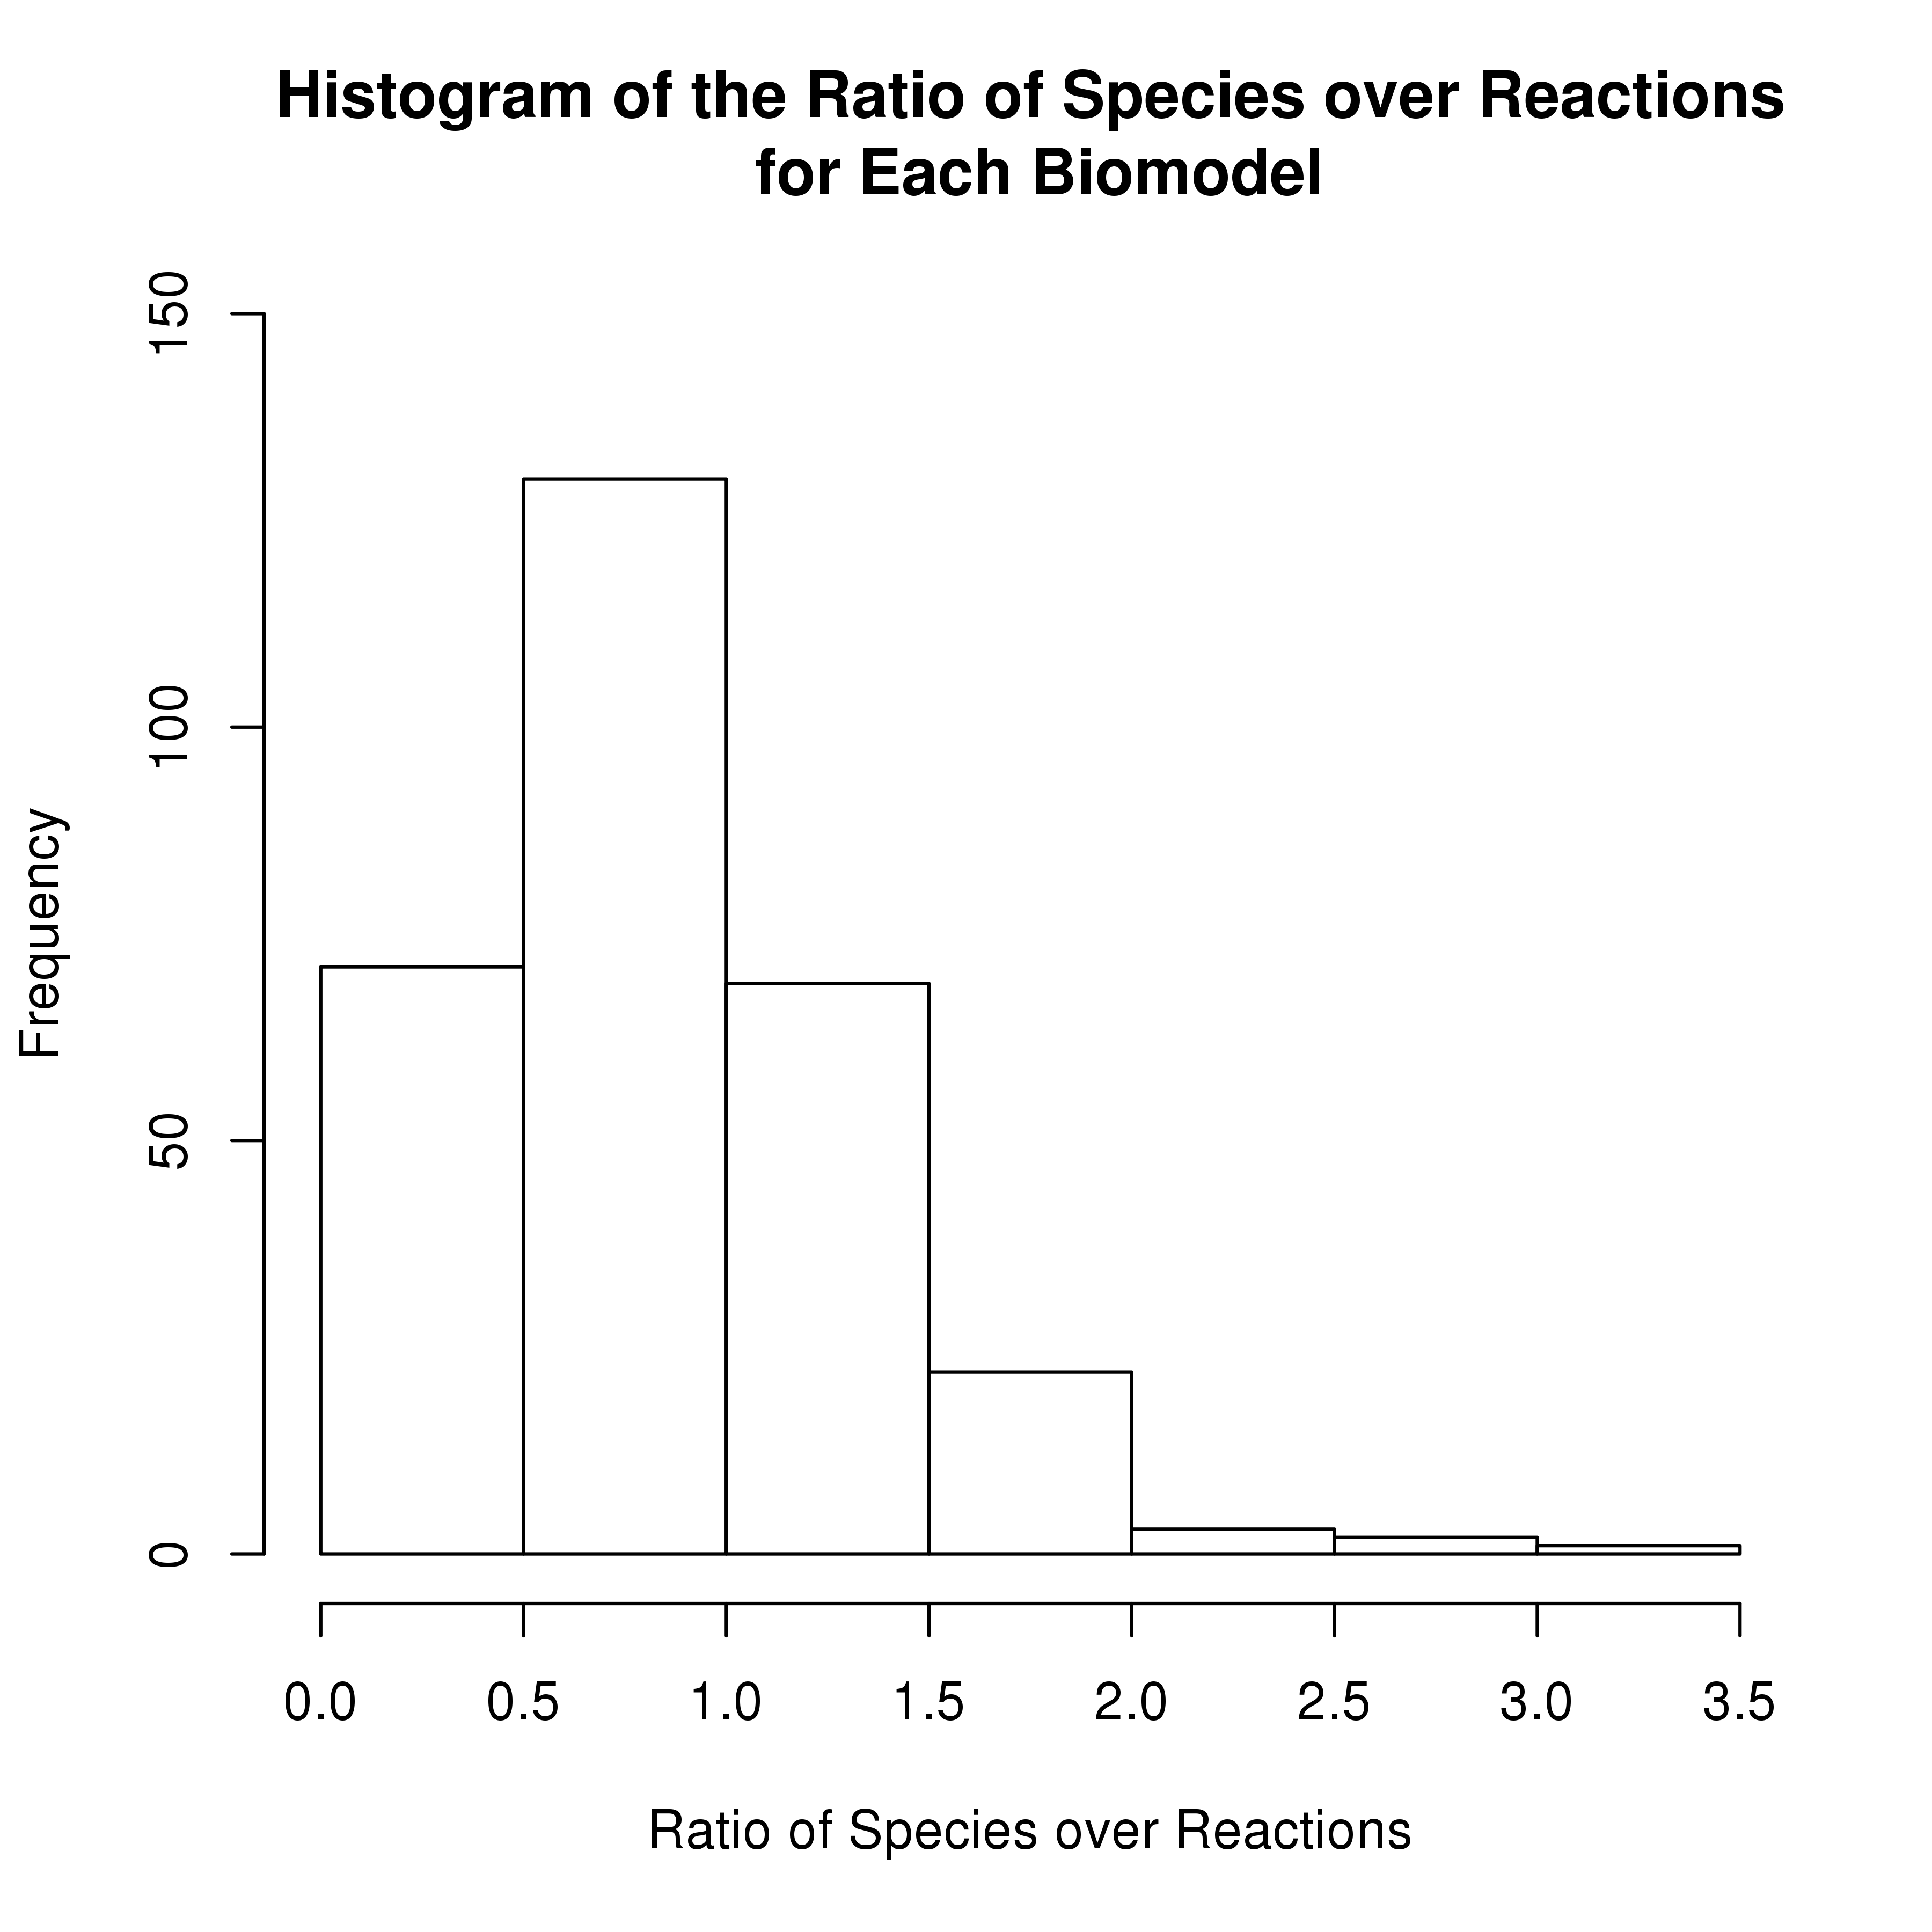
\includegraphics[trim= 1.5mm 5mm 5mm 5mm, clip, scale=0.42]{Poster-images/SpeciesOverReactions.png}}}
 {\flushleft{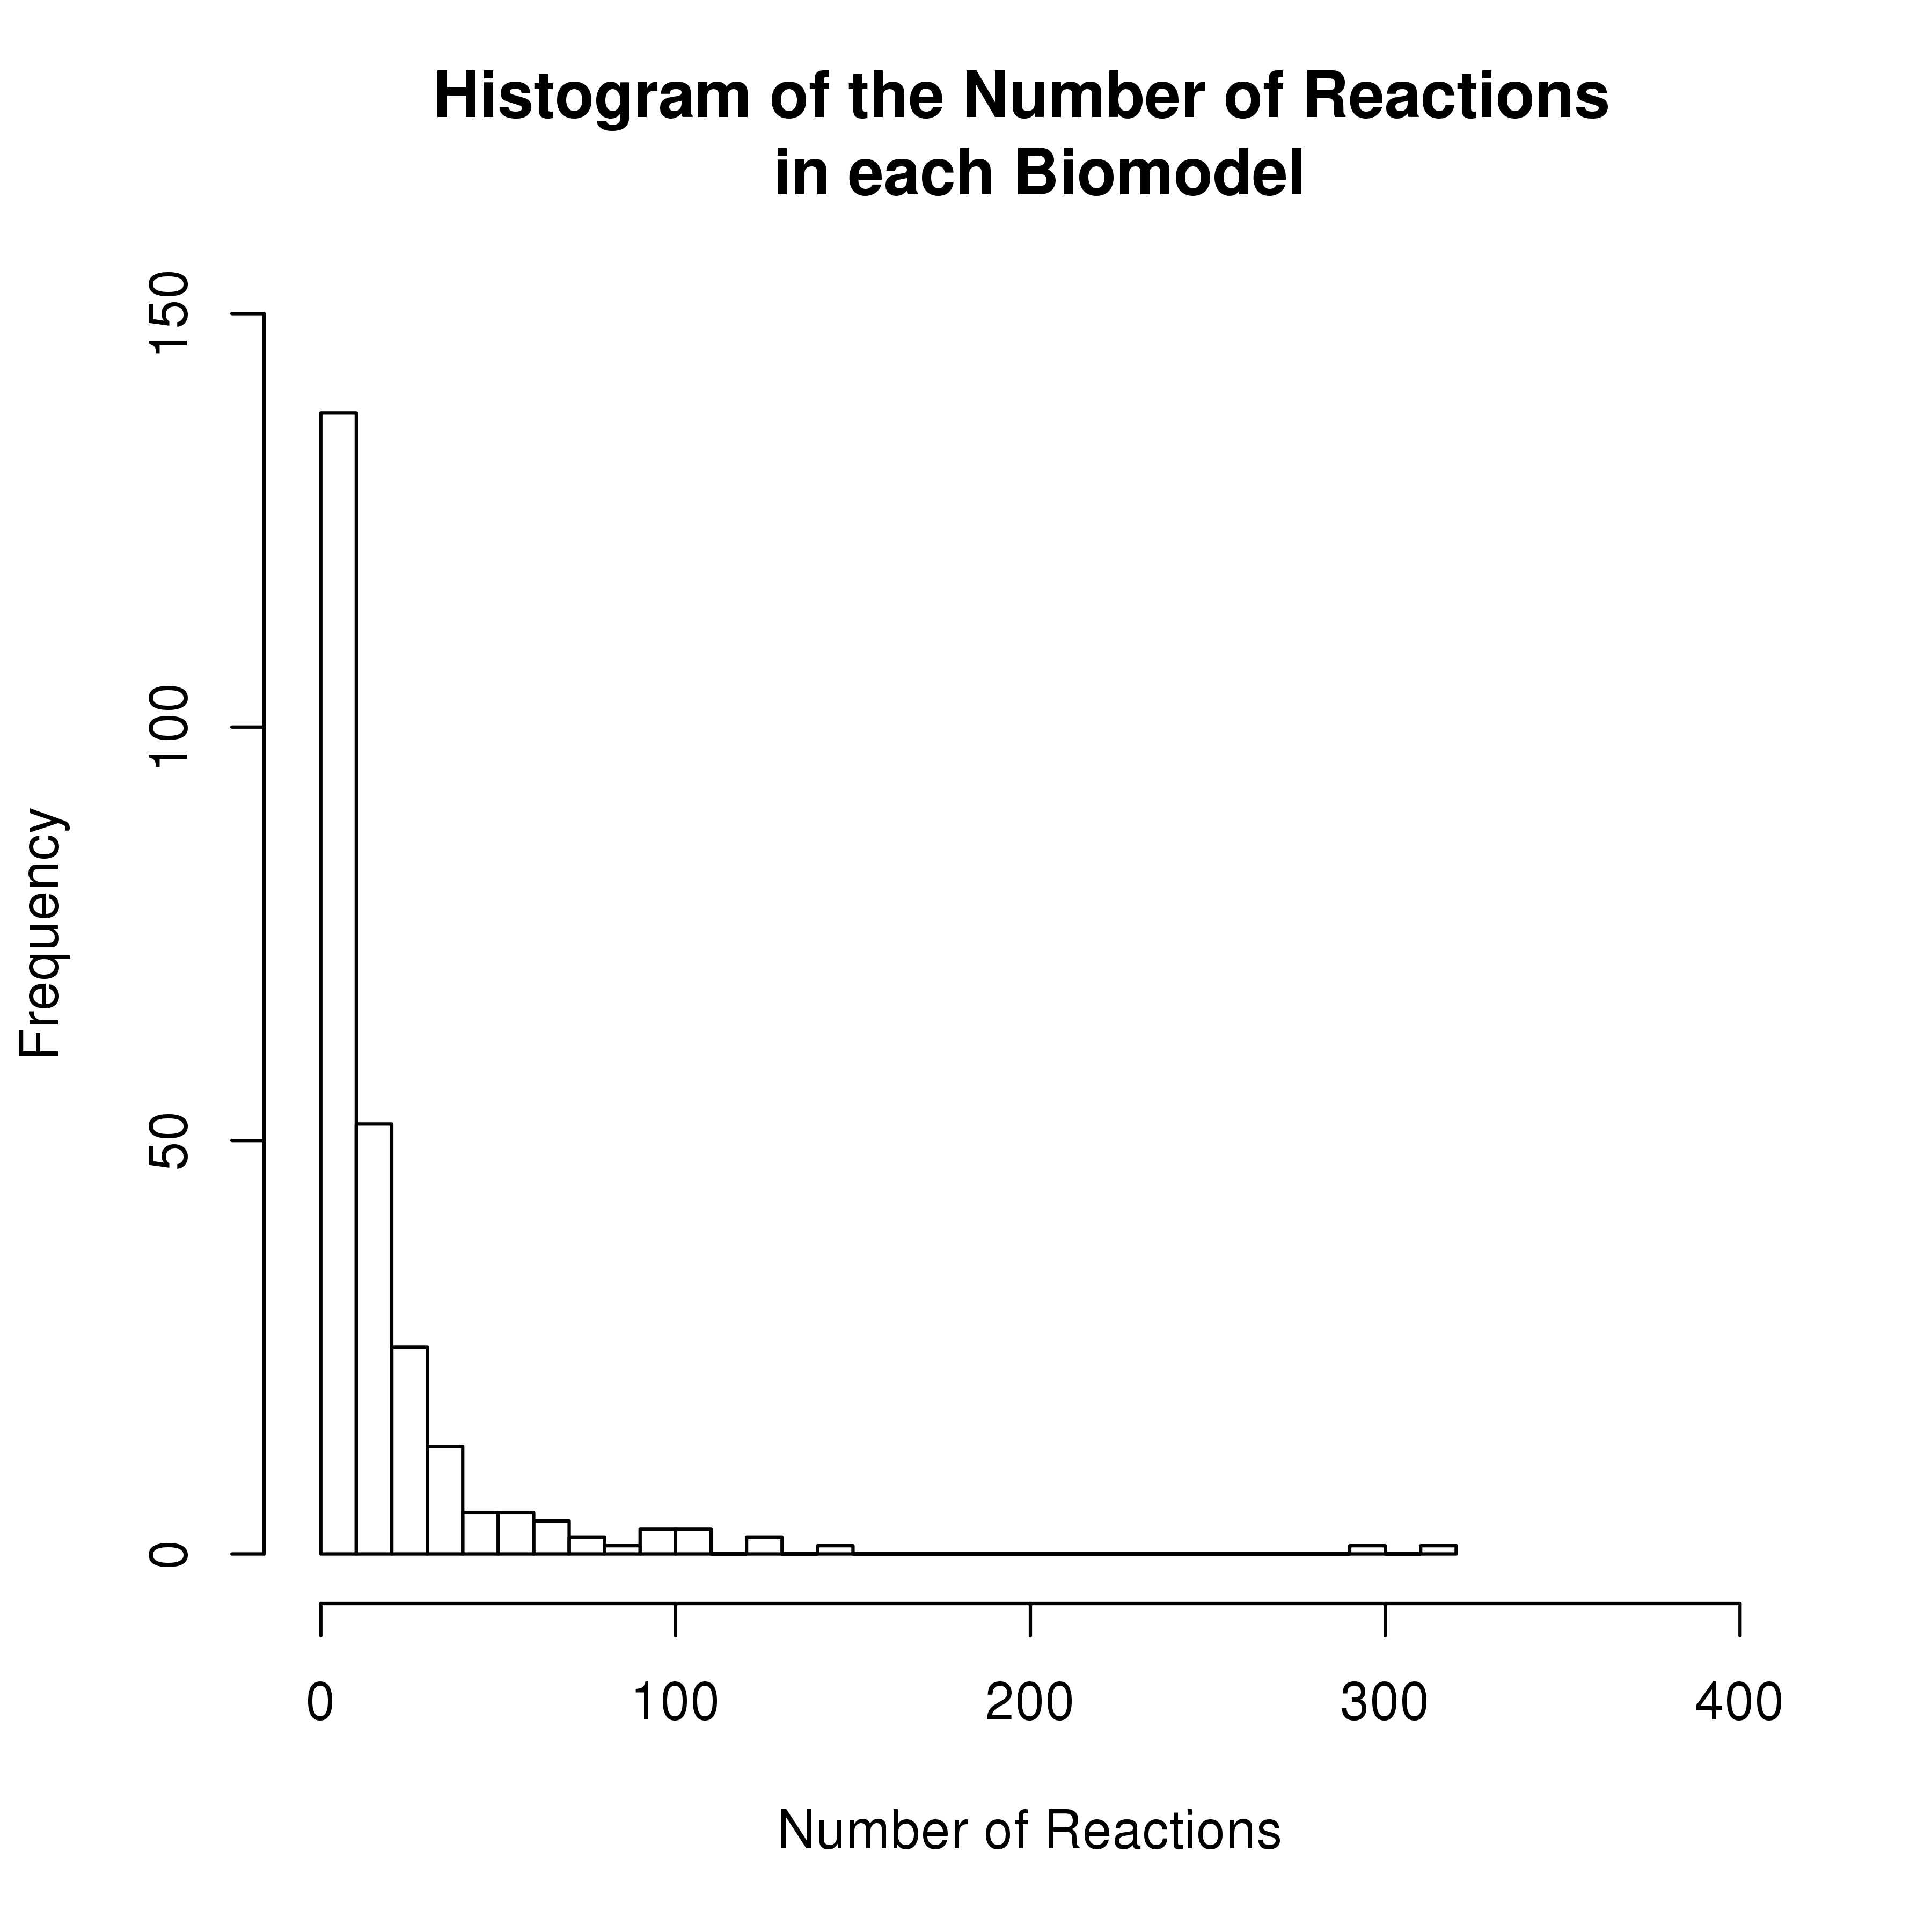
\includegraphics[trim= 1.5mm 5mm 5mm 5mm, clip, scale=0.42]{Poster-images/ReactionsHistogram.png}}}
 
  The species and reactions histograms have similar patterns, suggesting that the models tend to also have low numbers of reactions. \\
   
 The most frequent range of values for the ratios of species to reactions is 0.5-1.0, with the majority of models having ratios less than 2.
 
 This suggests that in the majority of models, the species tend to appear in multiple reactions, since if every species in a model appeared in just one reaction, the ratio would be at least 2.
 
 \end{multicols}
 }
 
\end{poster}

\end{document}